\documentclass[10pt]{article}

\usepackage{amsmath}

\newcommand{\myvec}[1]{\ensuremath{\begin{pmatrix}#1\end{pmatrix}}}

\newcommand{\mydet}[1]{\ensuremath{\begin{vmatrix}#1\end{vmatrix}}}

\newcommand{\solution}{\noindent \textbf{Solution: }}

\providecommand{\brak}[1]{\ensuremath{\left(#1\right)}}

\providecommand{\norm}[1]{\left\lVert#1\right\rVert}
\usepackage{graphicx}
\usepackage{float}

\let\vec\mathbf

\title{Coordinate Geometry}
\author{Charan(charan.n@sriprakashschools.com)}

\begin{document}
\maketitle
\section{Class 10$^{th}$ Maths - Chapter 7}
This is Problem-4 from Exercise 7.3
\begin{enumerate}
\item  QUESTION: Find the area of the quadrilateral whose taken in order are A(-4,-2), B(-3,-5), C(3,-2) and D(2,3).
\end{enumerate}
\solution \\We have two triangles ABC and ADC.\\
Then, \\Area of triangle ABC
\begin{align}
&=\frac{1}{2}\norm{{\vec{BA}\times \vec{BC}}}\\
&=\frac{1}{2}\mydet{ {-1}&{6}\\{3}&{3}}\\ 
&=\frac{1}{2}\norm{-3-18}\\
&=\frac{1}{2}(21)\\
&=\frac{21}{2} sq.units
\end{align}
\\Now, area of triangle ADC
\begin{align}
&=\frac{1}{2}\norm{{\vec{DA}\times \vec{DC}}}\\
&=\frac{1}{2}\mydet{ {-6}&{1}\\{-5}&{-5}}\\ 
&=\frac{1}{2}\norm{30+5}\\
&=\frac{1}{2}(35)\\
&=\frac{35}{2} sq.units
\end{align}
\\Now, Area of ABCD = Area of ABC + Area of ADC
\begin{align}
    &=\frac{21}{1}+ \frac{35}{2}\\
 &=28 sq.units
\end{align}

\begin{figure}[H]
			\centering
			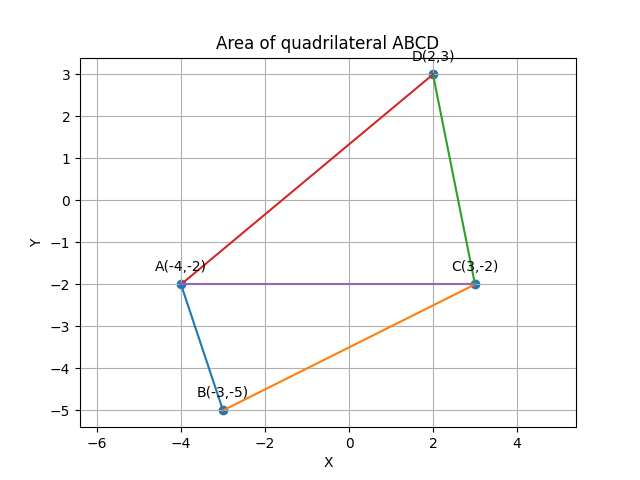
\includegraphics[width=\columnwidth]{figs/Figure_1.png}
			\caption{Quadrilateral ABCD}
			\label{fig:quad1}
		\end{figure}

\end{document}
